\chapter{Éthique de la modélisation intégrée}
\label{chapter:ethique}
\newrefsegment

\PEEL{Les modélisateur.ices ont une responsabilité vis à vis de ce que leurs modèles produisent. }{Fournissez des preuves, des données ou des citations qui soutiennent votre point.}{Expliquez en quoi les preuves que vous avez fournies sont pertinentes et comment elles appuient votre point.}{Faites le lien avec le sujet principal ou avec la section suivante de votre mémoire.}


\chapterabstract{Les choix de modélisation des fonctions de dommage sont lourds de conséquences sur le message que véhiculent les résultats de ces modèles. Ces résultats alimentent le débat public sur les questions climatiques. Vu les enjeux sociaux et sociétaux qui sont à l'oeuvre, la pratique de la modélisation implique des questions éthiques importantes. Quelles sont-elles, et comment sont-elles prises en compte ? Cette partie est plus conceptuelles et épistémiques, et cherche à identifer des points d'attention de la modélisation.}

\begin{quote}
    Dépolitiser le réel c'est le repolitiser au profit de l'oppresseur
\end{quote}


\begin{table}
    \centering
    \begin{tabular}{|c|c|c|c|} \hline 
         Pratique&  Enjeu&  Concept associé& Commentaire\\ \hline 
         Choisir les modèles pour faire tourner les scénarios&  Framing / possibility space&  & \\ \hline 
         Attribuer une valeur à un paramètre (taux d'actualisation)&  Equité intergénérationnelle&  & \\ \hline 
         Fabrique du doute&  Responsabilité dans l'interprétation des résultats&  Doute normativement inappropriés& \\ \hline
    \end{tabular}
    \legende{Enjeux éthiques dans les modèles et cadre d'analyse associés}{}
    \label{tab:ethique}
\end{table}


\cite{schienke_intrinsic_2011} => sur l'éthique intrinsèque dans les IAMs
\cite{weitzman_modeling_2009} => sur les evenements non-linéaires

\begin{tcolorbox}
    Voir Gouverner le climat !!
\end{tcolorbox}


\section{Les trois niveaux de l'éthique et la responsabilité du modélisateur}

Cette section pose plusieurs questions quant à la place de la technique et de la modélisation dans la cité. 

Elle s'appuie notamment sur \cite{jonas_principe_2008} et \cite{vast machine}, ainsi que sur la classification des enjeux éthiques de \cite{tuana_leading_2010}.


Comme nous l'avons vu précédemment, le processus de modélisation est avant tout un processus de sélection de ce qui est représenté et ce qui ne l'est pas, et de décision de la manière de le représenter. Comme nous le verrons dans le chapitre \ref{chapter:socio}, l'imperfection et la partialité des modèles est souvent assumée, voire revendiquée par les équipes de modélisation. Elle s'accompagne souvent d'une tentative de dé-responsabilisation de l'équipe de modélisation. Celle-ci prend généralement la forme suivante : 

\begin{quote}
    Les résultats des modèles sont valables uniquement sous les conditions (nombreuses et irréalistes) dans lesquelles il a été conçu. On ne peut donc pas extrapoler les résultats, ou faire dire au modèle autre chose que ce qu'il veut dire. 
\end{quote}
Pourtant, les résultats des modèles sont utilisés de manière large, notamment pour prendre des décisions de politique publique, y compris par des personnes n'ayant pas de compétence spécifique en modélisation, ni de connaissance particulière des modèles utilisés pour produire les connaissances qu'elles utilisent. Il y a donc un paradoxe : d'une part, l'idéal d'une compréhension fine des hypothèses de la modélisation, qui permet d'être conscient des choix de modélisation et de leurs implications. Cet idéal protège la responsabilité du modélisateur : en effet, les hypothèses ayant été clairement formulées, l'utilisateur final devient responsable de sa propre interprétation. Celle-ci se fait en accord avec les hypothèses énoncées, que l'utilisateur final fait sienne. D'autre part, il est difficile de comprendre un modèle pour plusieurs raisons : technique (les logiciels ne sont pas/plus accessibles), légales (le code source n'est pas accessible librement), capacitaires (les codes sources sont difficiles à interpréter, surtout si on n'est pas familier du langage utilisé), théoriques (les modèles intégrés font appel à des concepts issus de nombreuses disciplines). Cette difficulté à comprendre les modèles font que les résultats sont \textit{de facto} souvent interprétés dans l'état dans lequel ils sont délivrés, sans la contextualisation permise par le code. Dès lors, le choix des hypothèses est invisibilisé, et la responsabilité du modélisateur peut s'étendre jusqu'à l'interprétation du modèle, voire jusqu'aux conséquences de cette interprétation. \\

Pour éclairer ce paradoxe, nous allons nous intéresser aux dimensions éthiques de la modélisation. Pour cela, nous allons nous appuyer sur les travaux de Tuana, qui a cherché à developper un cadre conceptuel de l'éthique dans la recherche, et qu'elle a adapté spécifiquement au cas de la modélisation intégrée. \\

Elle développe trois dimensions éthiques de la recherche scientifique : l'éthique procédurale, l'éthique intrinsèque et l'éthique extrinsèque. 

\begin{figure}
    \centering

    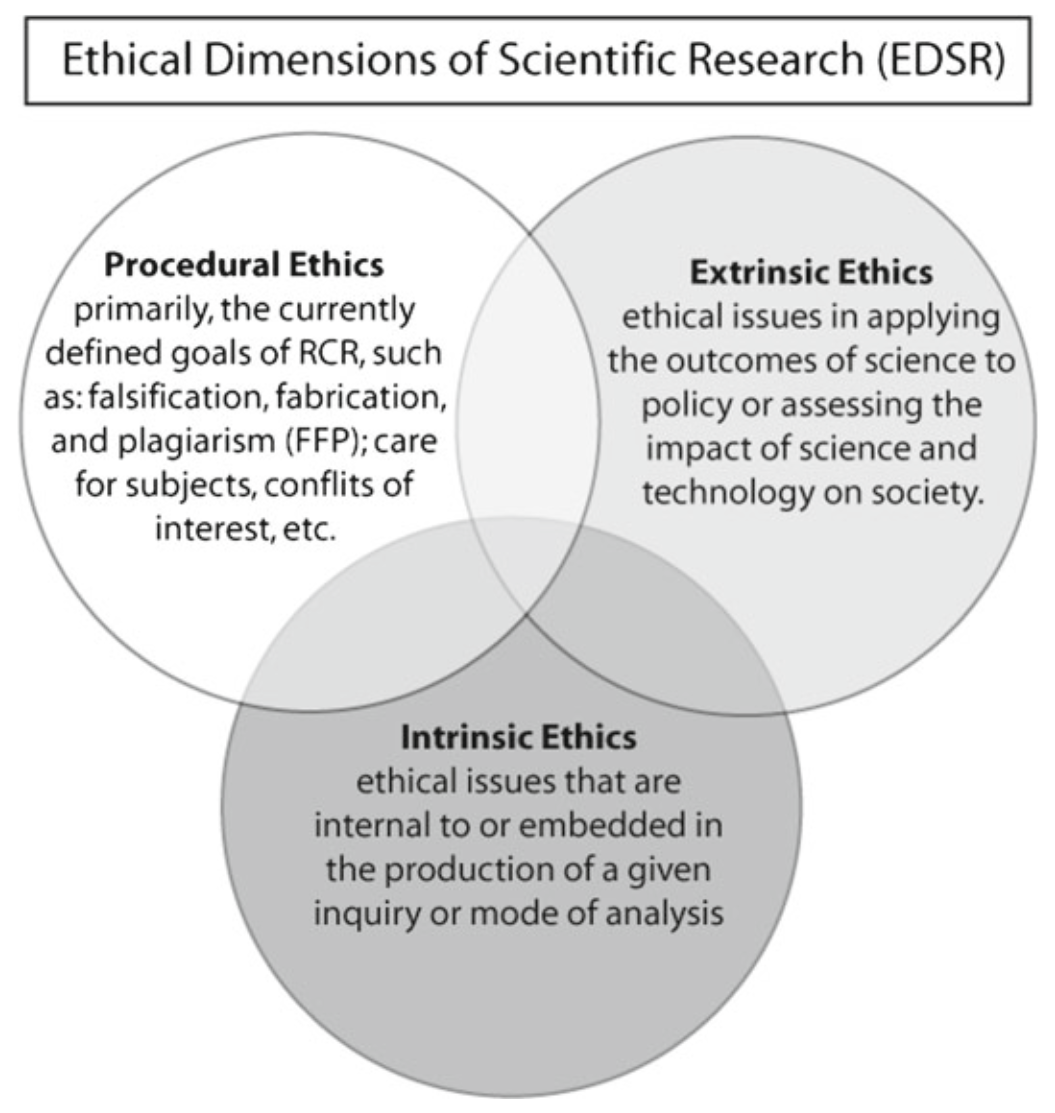
\includegraphics[width=1\linewidth]{venn_ethics.png}
    \legende{Les trois dimensions de l'éthique dans la recherche.}{\cite{tuana_climate_2019} décrit trois dimensions éthiques dans la recherche : l'éthique procédurale consiste en le respect des normes établies et reconnues dans la communauté. C'est en général ce à quoi on fait référence quand on parle de \textit{bonne science}. L'éthique extrinsèque désigne les questions éthiques qui sont liées aux utilisations des productions scientifiques. Enfin, l'éthique intrinsèque désigne les questions qui sont incluses dans le mode de production de la connaissance (en l'occurence, le modèle). }
    \label{fig:diag-venn}
\end{figure}


\subsection{L'éthique procédurale}

L'\Gls{procedural ethics} désigne ce qui est couramment regroupé sous le terme de \textit{bonne science}, ou \textit{good science}. Il s'agit de produire de la connaissance en respectant les attentes de la communauté scientifique en termes de honneteté, de sincérité. Tuana \cite{tuana_leading_2010}  la définit comme ceci : 

\begin{quote}
Ethical aspects of the process of conducting scientific research, such as: falsification, fabrication, and plagiarism; care for subjects (human and non-human animal); responsible authorship issues; analysis of and care for data.
\end{quote}
La plupart des travaux de modélisation s'inscrivent pleinement dans cette démarche, et sont en phase avec les attentes et bonnes pratiques de la communauté : 

\begin{itemize}
    \item tranparence : les codes sources sont ouverts et accessible, il y a une documentation plus ou moins complète
    \item honneteté : les hypothèses sont clairement énoncées
    \item sincérité des résultats : les résultats sont reproductibles facilement
\end{itemize}

\begin{tcolorbox}
    Mais remarques de Keen sur Nordhaus
\end{tcolorbox}

\subsection{L'éthique intrinsèque}

L'\Gls{intrinsic ethics} va plus loin dans l'exigence. Il s'agit de la dimension éthique qui est directement intégrée dans le processus de recherche : il ne s'agit plus de la forme de la recherche, mais du fond de la recherche. 

\begin{quote}
Ethical issues and values that are embedded in or otherwise internal to the production of scientific research and analysis. These involve ethical issues arising from, for example: the choice of certain equations, constants, and variables; analysis of data; handling of error, and degree of confidence in projections.
\end{quote}
Comme le souligne Tuana, la bonne prise en compte de ces questionnements nécessite d'avoir un accompagnement épistémologique au sein des équipes de recherche, c'est-à-dire de prendre en compte ces enjeux comme partie intégrante du développement du projet : \emph{the domain of intrinsic ethics will not be fully successful unless it includes the expertise of philosophers of science. It is only when this domain becomes a focus of our field, that the range of relevant issues and their ethical and epistemic significance will be fully appreciated.} 

\begin{tcolorbox}
    A développer : 
    \begin{itemize}
        \item choix du taux d'actualisation
        \item 
    \end{itemize}
\end{tcolorbox}

Un exemple d'éthique intrinsèque est le découpage par région. Les modèles se focalisent sur certaines régions plus que d'autres, sont calibrés sur certaines régions (où il y a par ailleurs des données plus nombreuses et de meilleure qualité), et sont donc bien plus pertinents pour décrire les phénomènes dans certaines régions plus que dans d'autres. 

\begin{figure}[htbp]
    \centering
    \begin{minipage}{0.45\textwidth}
        \centering
        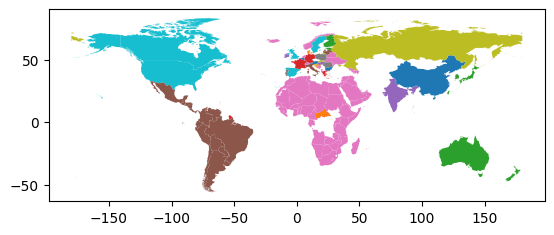
\includegraphics[width=\linewidth]{figures/FUND_regions.png} % Remplacez par le chemin de votre image
        \subcaption{FUND}
        \label{fig:carte1}
    \end{minipage}%
    \hfill
    \begin{minipage}{0.45\textwidth}
        \centering
        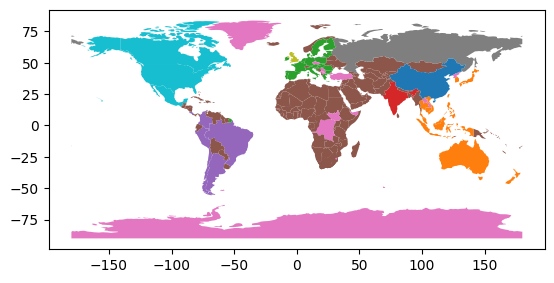
\includegraphics[width=\linewidth]{figures/WILIAM_regions.png} % Remplacez par le chemin de votre image
        \subcaption{WILIAM}
        \label{fig:carte2}
    \end{minipage}%
    \legende{Granularité spatiale différente entre les modèles}{}
    \label{fig:trois_cartes}
\end{figure} 



\subsection{L'éthique extrinsèque}

Enfin, l'\Gls{extrinsic ethics} désigne les questionnements autour des effets de la production scientifique sur la société. C'est une sphère beaucoup plus large, puisqu'elle sort du domaine du laboratoire et de la communauté scientifique, pour mesurer les effets sur les sociétés. 

\begin{quote}
Ethical issues that are external to the production of scientific research. These arise, for example, when considering the impact of scientific research on society; e.g., the effects of technological innovations on social ends such as health and well-being, whether pressing social and economic issues are likely to be addressed and if so, who benefits, and the role of science in policy-making. This domain of ethics also includes ethical concerns arising from the impact of society upon science, for example the impact of funding on research trajectories or the ways in which wide-spread societal biases can impact research trajectories, as they arguably did with eugenics research. In the latter case, there are often links between the domains of extrinsic and intrinsic ethics.
\end{quote}
Ce questionnement s'inscrit dans une réflexion plus large du rapport entre la production scientifique et son application dans la société. 

\begin{tcolorbox}
\begin{itemize}
    \item 
    \item [[cadrage]], forcément normatif « IAM analysis could focus on only a subset of relevant futures and thus push society in certain directions without sufficient scrutiny » (\href{zotero://select/library/items/2SDDNUUF}{“Annex III: Scenarios and Modelling Methods”, 2023, p. 1862}) (\href{zotero://open-pdf/library/items/CHVFSLLH?page=22&annotation=4MBM5B9Q}{pdf})

\end{itemize}

\end{tcolorbox}


 Ces considérations sur l'éthique extrinsèque prendront plus de sens dans la section suivante, on l'on développera l'idée que la modélisation participe activement au cadrage du débat public, et donc aux choix de futurs possibles. 

\section{Construire / dessiner les futurs possibles}

Cette section montre que le savoir produit par la science est situé dans le temps et dans l'espace. Ainsi, il n'est plus positif, mais bien normatif, en ceci qu'il décrit un univers des possibles. 

Un exemple de à quel point le framing peut impacter la connaissance est la classification des pays. Dans le SPM de l'AR5, les parties n'ont pas pu s'accorder sur un type de classification des pays à adopter ; finalement toutes les figures et textes associés ont été rejetées par les gouvernements. On pourrait ici penser que présenter une information ou une autre n'a pas d'importance, tant que celle-ci a été produite dans les normes scientifiques en vigueur. Pourtant, cet exemple montre que les gouvernements considèrent que le choix d'une classification porte en soi un message trop important ; reconnaissant alors l'absence de neutralité du contenu scientifique \cite{edenhofer_mapmakers_2014}. 

Les modèles intégrés sont utilisés comme base scientifique pour les négociations climatiques. Ils permettent notamment de décrire l'espace des possibles, c'est-à-dire l'ensemble des chemins qui peuvent être pris par les sociétés. Cette relation entre le modèle et la prise de décision est décrite par une image très parlante dans \cite{edenhofer_mapmakers_2014}, où les modélisateurs sont décrits comme des cartographes, et les décideurs comme des navigateurs. Dès lors, le rôle des modélisateurs-cartographe est de décrire l'espace possible, l'ensemble des zones qui sont navigables ; et, si possible, les conditions de navigation que l'on peut rencontrer dans ces zones.  En regard de ces nouvelles connaissances, les décideurs-navigateurs doivent décider du cap à suivre aujourd'hui selon la zone de navigation voulue pour demain. Cette distinction très nette entre décideurs et modélisateurs n'est pas sans limitations. L'une d'entre elle est le cadrage, c'est à dire la manière dont le débat public est façonné par le cadre qu'on lui donne.  Plusieurs choses influencent ce cadrage. Nous verrons d'abord que le prisme technique et énergétique aggrégé de la plupart des modèles représente ce genre de contraintes, sans questionner les modèles sous-jacents. Nous verrons ensuite que le choix des variables, et notamment la monétarisation des dommages fait que de nombreuses dynamiques ne sont soit pas prises en compte, soit prises en compte d'une manière que l'on peut questionner. Enfin, nous, aborderons l'idée que la connaissance est socialement construite, en se basant notamment sur les écrits de Helène Ongino, pour questionner le caractère universel des résultats des modèles. 

\subsection{Un monde homogène, technique et neutre ?}

=> il n'y a pas de modèle qui décompose les dommages par groupe sociaux

Helene Longino va plus loin dans sa critique de la science neutre en s'inscrivant dans une perspective d'épistémologie néo-marxiste. Elle met en avant trois points principaux : les conséquences du progrès technique, qui découle de la science, les travers du réductionnisme, et la possibilité d'une science plus émancipatrice. Cette approche remet les enjeux de rapport de force au cœur de l'épistémologie, et permet d'avoir une lecture politique de la production scientifique. \\

D'abord, elle clame que les dérives du progrès technique sont les inévitables conséquences de la production scientifique. 

\begin{quote}
    One is that the dystopic applications of modern science—the domination of political life by thermonuclear weapons, new particle beam weapons, and other monsters of annihilation; the control of human potentiality through genetic engineering; the proliferation of toxic wastes from science-based technologies; the displacement of human labor by automation—are not a misuse of socially neutral science but the inevitable result of bourgeois science.
\end{quote}

« there are concerns that IAMs are describing transformative change on the level of energy and land use, but are largely silent about the underlying socio-cultural transitions that could imply restructuring of society and institutions » (\href{zotero://select/library/items/2SDDNUUF}{“Annex III: Scenarios and Modelling Methods”, 2023, p. 1862}) (\href{zotero://open-pdf/library/items/CHVFSLLH?page=22&annotation=JY4VBIZY}{pdf})



=> extrait sur le réductionnisme.

\begin{figure}
    \centering
    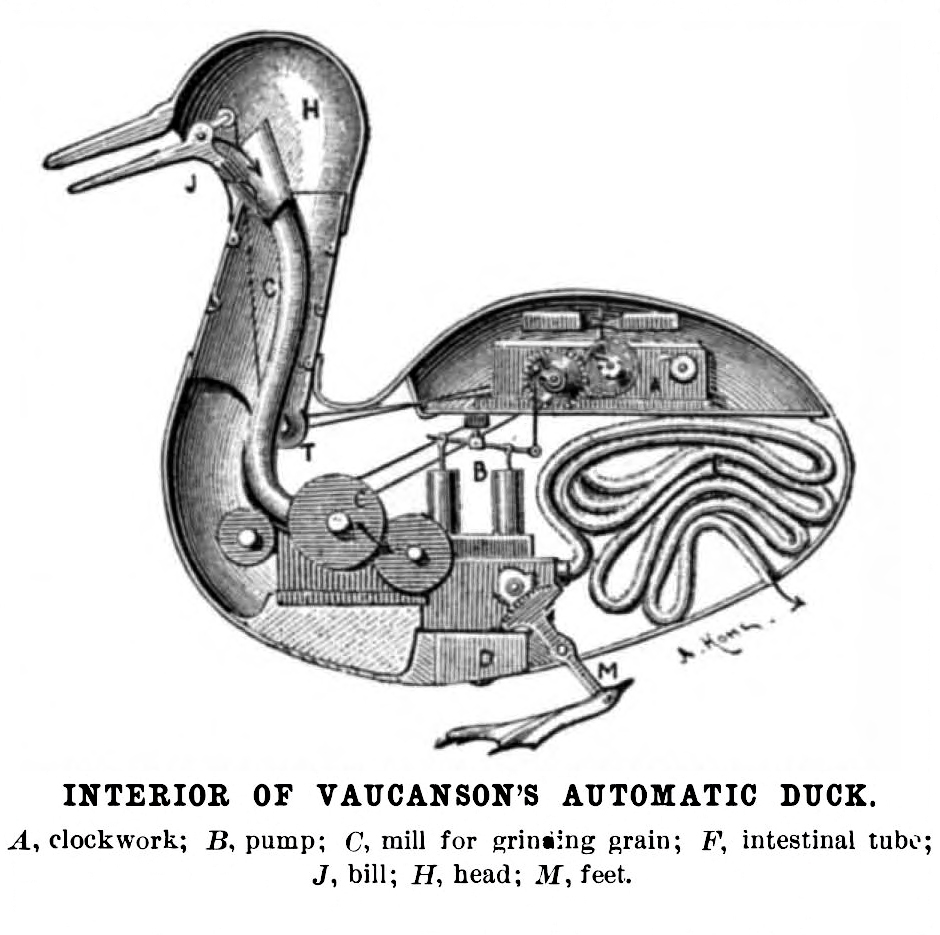
\includegraphics[width=0.75\linewidth]{reductionisme.png}
    \legende{Modèle d'un canard dans une perspective réductioniste}{Le réductionisme tend à décrire les phénomènes par des lois physiques.}
    \label{fig:reductionnisme}
\end{figure}

\begin{quote}
    
\end{quote}

L'autrice continue sa critique en formulant un rejet du réductionnisme, c'est-à-dire à la croyance selon laquelle une notion peut être réduite en d'autres notions plus fondamentales. Elle appelle à une conception plus systémique des des relations causales. 

\begin{quote}
    The spirit, therefore, of these analyses might be better served by seeing them as urging a reconception of objects of inquiry in particular fields — specifically as urging their colleagues to abandon questions presupposing unidirectional or linear causal relations and to understand objects as constituted partly of the parts of which they are wholes and partly of the wholes of which they are parts. If this shift could be accomplished on internalist grounds, there would be less struggle over its acceptance.
\end{quote}

Ce point touche tout à fait les modèles, et particulièrement les fonctions de dommage. Les modèles sont une forme de réductionnisme, puisque l'on représente des phénomènes complexes à travers des fonctions plus simples. Il s'agit donc d'une critique récurrente, mais dont il convient de faire attention. \\


Une autre difficulté rencontrée par les modèles est la représentation des altérités et des différences. Les modèles tendent à décrire un monde homogène et neutralisé. En effet, les régions sont similaires; elles ont certe des paramétrisation différentes, mais les mécanismes décrits sont les mêmes. On gomme par là les différences culturelles et institutionnelles entre les différentes régions du monde. \\

\begin{tcolorbox}
    Partie sur Aykut et Dahan
\end{tcolorbox}

Ces critiques rejoignent celles formulées par Aykut et Dahan. 

\begin{quote}
    Au cours des années 1990, les pays en développement ne sont convaincus ni de la gravité du risque climatique ni du fait que ce problème les concerne. Ils contestent la prééminence de son traitement « physique » qui privilégie trop, selon eux, le global par rapport au local. Ils critiquent le point de vue de la modélisation numérique globale ou, du moins, le transfert de sa méthodologie au niveau politique ; transfert qui, disent-ils :  
    \begin{itemize}
        \item effacerait le passé (or, le Nord s’est industrialisé, équipé et il a pollué, pas le Sud)
	    \item naturalise rait le présent (en particulier, la référence à l’année 1990 dans le protocole de Kyoto est jugée inacceptable, le présent n’étant pas un acquis, mais devant être interrogé),
	   \item et globaliserait le futur (le CO 2 se globalise sans doute, pas les humains).
    \end{itemize}
\end{quote}

Si cette critique concerne principalement les modèles physiques tels que les modèles de circulation générale, ils peuvent être apportés également aux modèles intégrés. En effet, dans les modèles d'optimisation, où le coût total est minimisé, l'origine des émissions ou le lieu des dommages n'importe pas. 


 \subsection{Prendre en compte le non-monétaire}


« The difficulty in fully representing the extent of climate damages in monetary terms may be the most important and challenging limitation of IAMs and it is mostly directed to costbenefit IAMs. However, all categories of IAMs present important limitations (Annex III.I.9). » (\href{zotero://select/library/items/2SDDNUUF}{“Annex III: Scenarios and Modelling Methods”, 2023, p. 1844}) (\href{zotero://open-pdf/library/items/CHVFSLLH?page=4&annotation=YT933ZM4}{pdf})
 

\begin{itemize}
    \item « there are concerns that IAMs are missing important dynamics » (\href{zotero://select/library/items/2SDDNUUF}{“Annex III: Scenarios and Modelling Methods”, 2023, p. 1861}) (\href{zotero://open-pdf/library/items/CHVFSLLH?page=21&annotation=WDMBNU3A}{pdf})
=> et donc ne sont pas vraiment précis, ou passent à coté de certaines choses

\end{itemize}


Enfin, l'approche néomarxiste fait la promotion d'une science plus émancipatoire, et moins élitiste. Longino évoque notamment les travaux de Hilary Rose et Steven Rose, qui décrivent une science plus émancipatoire, qui aurait \emph{dépassé le clivage entre l'objet et le sujet, entre le rationnel et l'emotionnel, et qui ne serait plus dominée par une rationalité instrumentale. Elle serait caractérisée par des relations sociales démocratiques, c'est-à-dire l'abandon de l'élitisme, et ses théories incorporeraient une vue dialectique de la nature}.


\subsection{Le cadrage : dans la lumière ou dans l'ombre du projecteur}
% \subsection{La modélisation, une connaissance construite}

- « On peut résumer les trois modalités essentielles par lesquelles les sciences du climat ont influencé les politiques :  
	- la **concentration sur les modèles globaux de l’atmosphère** comme outil incontournable des projections climatiques, y compris pour les prévisions régionales obtenues par descente en échelle (downscaling) des modèles globaux, a contribué à globaliser les problèmes, à désigner l’arène mondiale/globale comme l’échelle unique de traitement du risque climatique ;
	- le **réductionnisme physico-chimique des sciences du climat** tend à mettre en avant les caractéristiques universelles des GES et à les séparer de leur signification sociale locale. Les molécules de méthane des rizières ou celles de gaz carbonique des voitures jouent un rôle identique dans la mise en équation de l’effet de serre. C’est ce que Demeritt (2001) a qualifié de déterminisme environnemental tacite ;
	- la **focalisation dans les modélisations sur les « évolutions probables »** a longtemps contribué – contrairement à ce que les critiques récurrentes de « l’alarmisme » des rapports scientifiques suggèrent – à une marginalisation des scénarios du pire et de l’éventualité de changements brusques, ou tipping points. Shackley et Wynne (1996) constatent, dans une étude sur le traitement des incertitudes dans l’expertise climatique globale, une « mise à l’écart des extrêmes » (tuning out of extremes). » ([Aykut et Dahan, 2014, p. 19]
		- Shackley et wynne

C'est également ce que l'on peut qualifier de globalisme du climat. 


\begin{tcolorbox}
    parler du fait que l'optimisation c'est forcément très normatif. 
\end{tcolorbox}

\section{Les doutes normativement inappropriés, ou la limite entre mauvaise science et fabrique de l'inaction}

Cette section repose sur les approches des \textit{ignorance studies}, notamment \cite{melo-martin_fight_2018} et \cite{gross_routledge_2015}, avec comme ressources complémentaires \cite{noauthor_carnet_2024} et \cite{proctor_agnotology_2008}. Elle est tirée de réflexions tirées du cours de Mathias Girel à l'ENS \cite{girel_vertus_2023}. 



+ Stern / Nordhaus argument (c'est sûr qu'ils se sont balancé des trucs à la gueule) 

+ steve keen \cite{keen_appallingly_2021}

\subsection{Rester dans sa retenue ou s'engager ?}

\subsection{L'impossible neutralité des modèles}

Helène Longino définit deux types de valeurs. D'une part, les \emph{constitutive values}, qui désignent les valeurs méthodologiques admises par la comunauté, c'est-à-dire les bonnes pratiques et méthodes. D'autre part, les \emph{contextual values}, qui sont des valeurs personnelles, sociales ou contextuelles des individus. Ces valeurs sont plus normatives, et reflètent le cadre social et culturel dans lequel s'inscrit la démarche scientifique. \\

Se pose dès lors la question du rapport entre ces deux niveaux de valeurs. Dans quelle mesure les valeurs contextuelles influencent les valeurs constitutives, c'est-à-dire dans quelle mesure les normes sociales d'un contexte donné vont influencer la production scientifique ? Et dans quelle mesure les valeurs constitutives influencent les valeurs contextuelles, c'est-à-dire dans quelle mesure la production scientifique influence les normes sociales ? Cette question est celle de l'autonomie de la pratique scientifique du contexte personnel, social et culturel, c'est-à-dire précisément la question de la neutralité de la science. Elle répond de manière très claire à cette question : non seulement les deux interagissent fortement, mais cette interaction est au cœur de la pratique scientifique : 

\begin{quote}
    I will argue not only thatscientific practices and content on the one hand and social needs and values on the other are in dynamic interaction but that the logical and cognitive structuresofscientific inquiry.require such interaction. \textit{p. 5}
\end{quote}

L'autonomie de la production scientifique vis-à-vis des valeurs sociales est donc un mythe. Cependant, et contrairement à ce qui est généralement admis, cela ne remet pas en cause l'intégrité de la recherche. 

\begin{quote}
    Autonomy and integrity are separable attributes, and I shall consider them in sequence.
\end{quote}

La question de la neutralité de la science est régulièrement abordée en épistémologie. Une autrice a particulièrement abordé ce sujet, en montrant que la science est avant tout une pratique sociale, qui s'inscrit dans des dynamiques et un contexte particulier. Il s'agit d'Hélène Longino, dans \emph{Science as social knowledgde} \cite{longino_science_1990}. Elle développe plusieurs points qui vont être intéressants dans la perspectives des modèles. \\

D'abord, elle développe l'idée que la science n'est pas pure ou dénuée de valeur; au contraire, c'est une base solide pour construire des valeurs ensuite. Il ne s'agit pas de lutter pour une science sans biais ou sans valeur; mais plutot d'inclure ces valeurs au coeur du projet scientifique. 

\begin{quote}
    Instead of remaining passive with respect to the data and what the data suggest, we can, therefore, acknowledge our ability to affect the course of knowledge and fashion or favor research programs that are consistent with the values and commitments we express in the rest of our lives. From this perspective the idea of a value-free science is not just empty but pernicious. \textit{page 191}
\end{quote}

Elle va ensuite plus loin, en indiquant qu'il y a un choix fort à réaliser, entre s'accorder avec les systèmes normatifs traditionnels, ou s'accorder avec son propre système de valeurs. Le système normatif, qui est forcément inclu dans le processus scientifique, résulte dès lors d'un choix conscient (y compris s'il implique de rester dans le système de valeur traditionnel ou dominant). 

\begin{quote}
    In particular we can choose between being accountable to the traditional establishment or to our political comrades \textit{p 191}
\end{quote}

Le contexte de la modélisation est particulièrement intéressant de ce point de vue. En effet, comme nous l'avons montré plus haut, les hypothèses sont omniprésentes, et réflètent une conception du monde. Il y a donc un choix réel. Contrairement à ce que certains modélisateurs affirment, il ne s'agit pas d'une réalité objective ou neutre, mais bien d'une sélection hautement normaitve. \\




\cite{helgeson_attention_2022} => pote de Tuana qui parle des valeurs

\subsection{La responsabilité}




